%          spconf.sty  - ICASSP/ICIP LaTeX style file, and
%          IEEEbib.bst - IEEE bibliography style file.
% --------------------------------------------------------------------------
\documentclass{article}
\usepackage{spconf,amsmath,graphicx,tabularx}
\usepackage{booktabs}

\usepackage{hyperref}

% Title.
% ------
\title{Applied machine learning system ELEC0134 22/23 report}
\name{SN: 12345678}
\address{}
%
\begin{document}
%
\maketitle
%
\begin{abstract}
    This section provides a brief overview of the methodology/results presented in the report.\footnote{The code is provided link-to-download-your-project.com and GitHub project: \href{http://www.google.com}{link-to-your-github-project}}
\end{abstract}
%
\begin{keywords}
    One, two, three, four, five
\end{keywords}
%

\section{Introduction}
\label{sec:intro}
    This section introduces the problem, a brief bird's-eye view of the methodologies you adopted and the organization of this report.
    
    A citation example is given here \cite{C2}. Use IEEE citation format.


\section{Literature survey}
\label{sec:lite}
    This section should focus on an overview of potential approaches to solve the tasks. You can introduce some classical and state-of-the-art machine learning algorithms.


\section{Description of models}
\label{sec:models}
    In this section, you should briefly describe the model you are using for each task, along with the rationale. You may opt to use a single learning algorithm to solve the problem or multiple ones, but bear in mind there are page limitations and that you should explain your rationale behind your choices. That is, the algorithmic description must detail your reasons for selecting a particular model.
    
    You can clarify them with flow charts, figures or equations. An example of how to draw an image is demonstrated in Fig. \ref{fig:roberts_building}.
    
    \begin{figure}[htb]
    \centering
    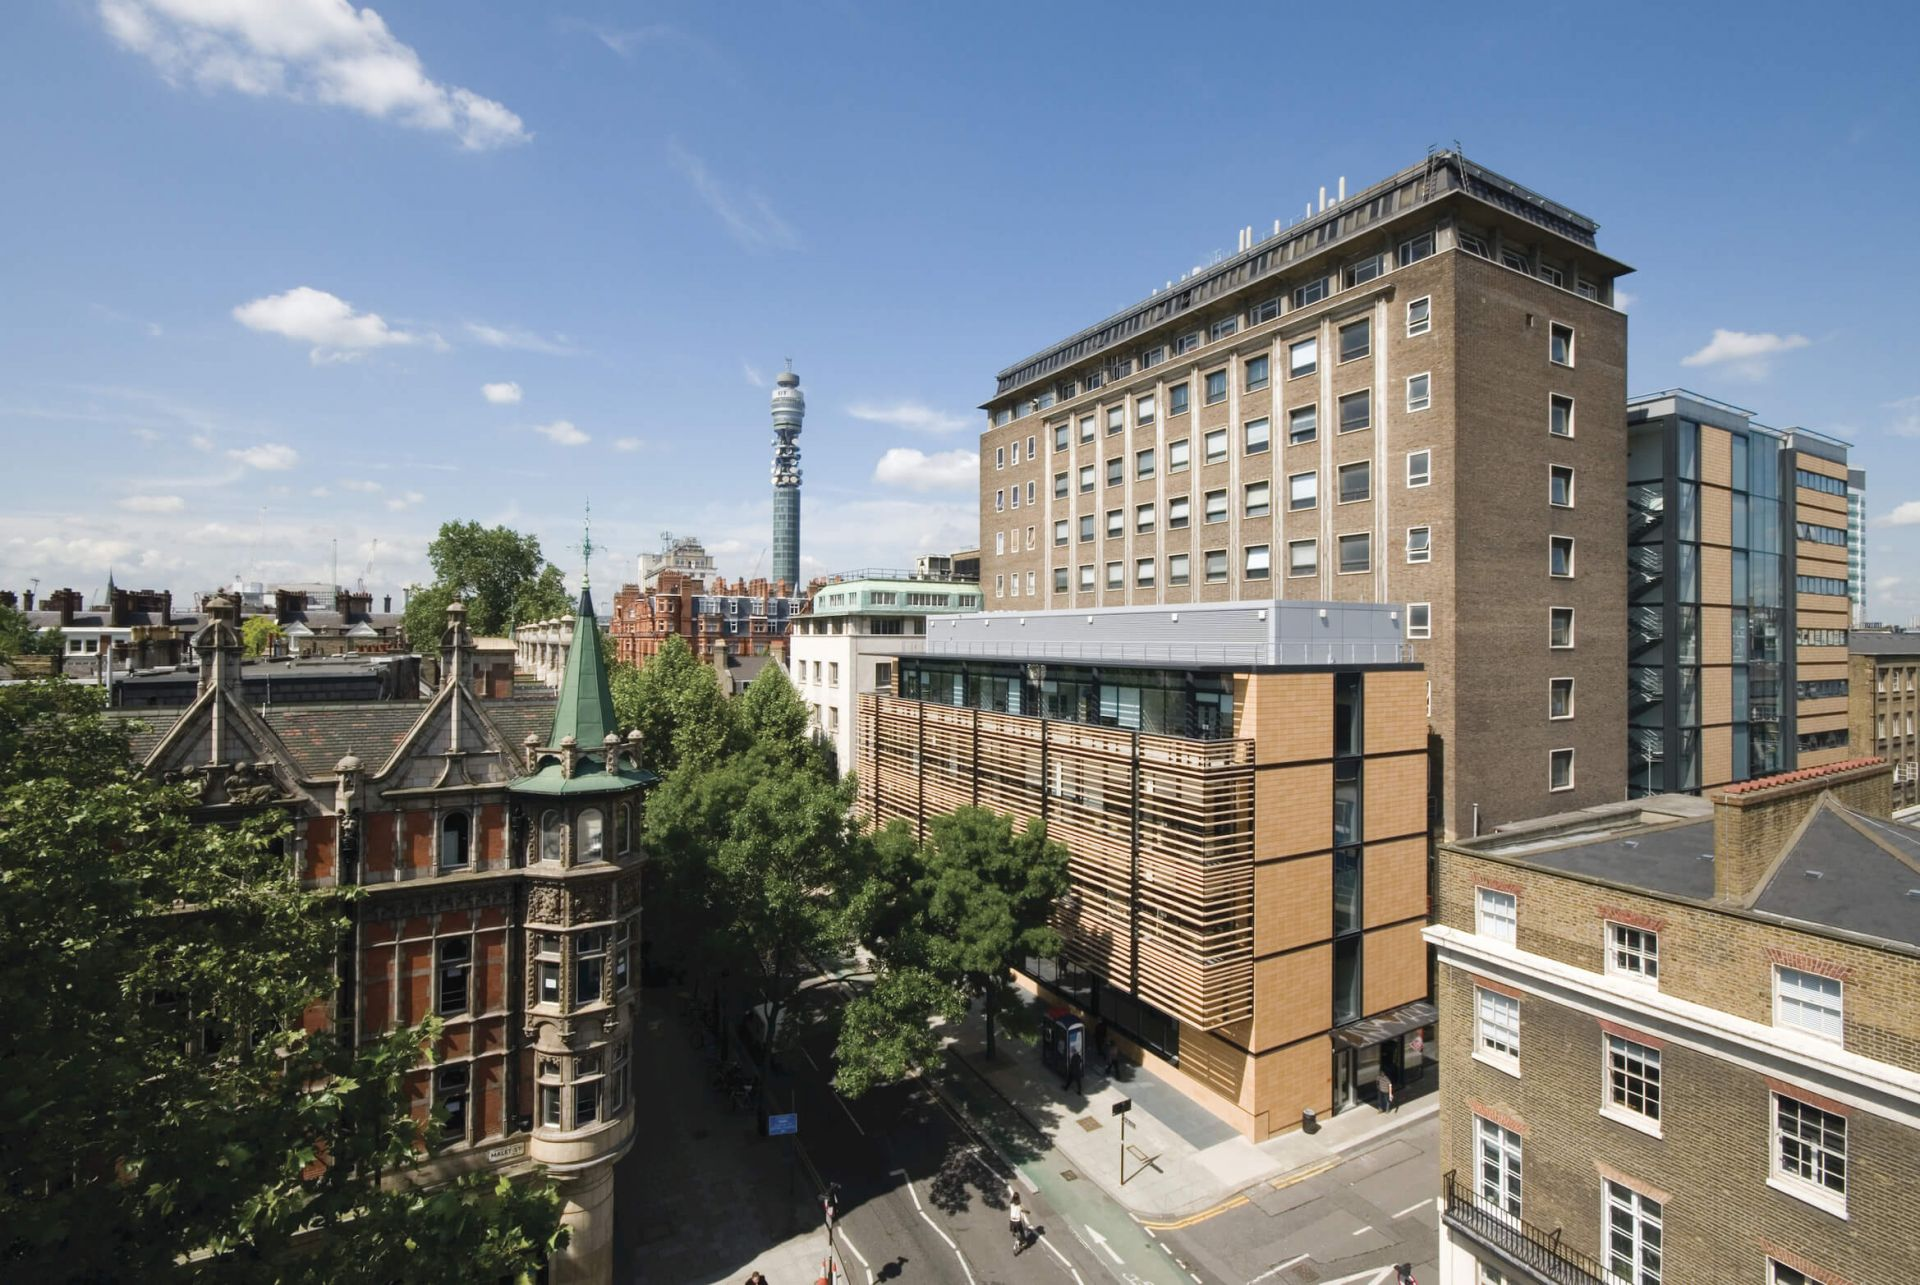
\includegraphics[width=0.48\textwidth]{images/Roberts_building.jpg}
    \caption{A nice view of Roberts Building}
    \label{fig:roberts_building}
    \end{figure}
    
    \subsection{Task A: the task name}
    \label{ssec:models_A}
    Hello world!
    \subsection{Task B: the task name}
    \label{ssec:models_B}
    Hello world!

\section{Implementation}
\label{sec:impl}
    This section must provide the detailed implementation of your models. In particular, you must provide the name and use of external libraries, explain hyper-parameter selection, training pipeline (if any) and key modules/classes/functions/algorithms.
    
    You also must provide a detailed description of the dataset (content, size, format, etc.), any data pre-processing that was applied and how you separate your dataset into training, validation and test sets.
    
    The execution of your models also should be reported here. In particular, this section should include a thorough discussion on the training convergence and stopping criterion (it is recommended that learning curves graphs be used to this effect).

    \subsection{Task A: the task name}
    \label{ssec:impl,models_A}
    \subsubsection{module name}
    Hello world!
    \subsection{Task B: the task name}
    \label{ssec:impl,models_B}
    Hello world!

\section{Experimental Results and Analysis}
\label{sec:results}
    This section describes and discusses your results. Additionally, this section should include accuracy prediction scores on a separate test dataset, provided by the module organizers, but not used during your training and validation process.
    
    We recommend you use a table to list the tasks, models and results before analysis.
    
    \begin{table}[h]
    \centering
    \label{table:Table1}
    \caption{Example of Table}
    % \begin{tabular}{0.48\textwidth}{lllll}
    \begin{tabular}{lllll}
    \toprule
           &  Col1 &   Col   &   Col3  &  Col4 \\ 
    \midrule
    Row1  &       &         &         &          \\
    Row2  &       &         &         &          \\
    Row3  &       &         &         &          \\
    Row4  &       &         &         &          \\ 
    \bottomrule
    \end{tabular}
    \end{table}

\section{Conclusion}
\label{sec:conc}
    This last section summarizes the findings and suggests directions for future improvements.


% References should be produced using the bibtex program from suitable
% BiBTeX files (here: strings, refs, manuals). The IEEEbib.bst bibliography
% style file from IEEE produces unsorted bibliography list.
% -------------------------------------------------------------------------
\bibliographystyle{IEEEbib}
\bibliography{refs}

\end{document}
